\section{Overview of Dataset}

\begin{table}
	\centering
	\caption{Frequency of some Tweet Objects  (for 1 million tweets) }
	\begin{adjustbox}{width=\columnwidth,center}	
	
	\begin{tabular}{|c|c|c|l|} \hline
		Object Name &Parent Object &Frequency&AVG Length(byte)\\ \hline
		tweet  & root object& 1,000,000 & 6599.305602\\ \hline
		users & tweet & 1,000,000 & 1453.798722\\ \hline
		coordinates  &tweet& 1586 & 57.87705\\ \hline
		place & tweet & 11974 & 392.8976115\\ \hline
		quoted status  & tweet & 177537 & 3993.947594\\ \hline
		retweeted status  & tweet & 598517 & 4775.996797\\ \hline
		entities  & tweet & 1,000,000 &336.02128\\ \hline
		extended entities  & tweet & 51479 & 1133.00505\\ \hline
		hashtags  & entities & 398720 & 44.0340615\\ \hline
		media  & entities & 51481 & 762.556516\\ \hline
		urls  & entities & 417176 & 187.6829563\\ \hline
		user mentions  & entities & 1063216 & 126.845482\\ \hline
		symbols  & entities & 7793 & 36.55832\\ \hline
		sizes  & media & 7793 & 36.55832\\ \hline
		media sizes  & sizes & 51485 & 194.91743\\ \hline
		thumb  & media sizes & 51485 & 37.989\\ \hline
		large  & media sizes & 51485 & 37.524\\ \hline
		medium  & media sizes & 51485 & 37.412\\ \hline
		small  & media sizes & 51485 & 36.993\\ \hline
		\hline\end{tabular}
		\end{adjustbox}
\end{table}


\begin{figure*}
	\centering
	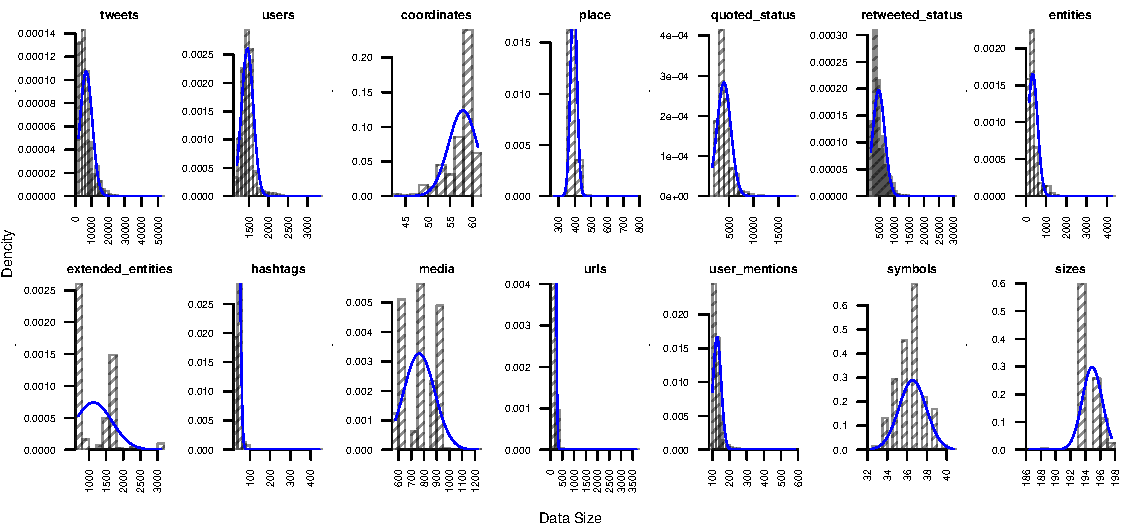
\includegraphics[scale=1]{img/Data_Overview.pdf}
	\caption{histograms with Standard Deviation}
	\label{fig:fly}
\end{figure*}